\documentclass{article}

\usepackage[T2A]{fontenc}
\usepackage[utf8]{inputenc}
\usepackage[russian, english]{babel}
\usepackage[left=2.3cm, right=2.3cm, top=2.7cm, bottom=2.7cm, bindingoffset=0cm, margin=3in]{geometry}
\parindent 0pt
\parskip -5pt
\usepackage{amsmath}
\usepackage{amssymb}
\usepackage{amsfonts}
\usepackage{amsthm}
\usepackage{graphicx}
\usepackage[shortlabels]{enumitem}
\usepackage[all]{xy}
\usepackage[usenames]{color}
\linespread{1.3}


\usepackage{color}
\usepackage{listings}
\definecolor{mygreen}{rgb}{0,0.6,0}
\definecolor{mygray}{rgb}{0.5,0.5,0.5}
\definecolor{mymauve}{rgb}{0.58,0,0.82}
\definecolor{myorange}{rgb}{0.855,0.576,0.027}
\lstset{
    language=Octave,
    basicstyle=\ttfamily,
    frame=tb,
    extendedchars=\true,
    morecomment = [l][\itshape\color{blue}]{\%},
    keywordstyle=\color{blue},
    commentstyle=\color{mygreen},
    breakatwhitespace=false,         
    breaklines=true,  
    numbers=left,
    numbersep=-10pt,
    numberstyle=\tiny\color{mygray}, 
    showstringspaces=false,
    showtabs=false,                  
    tabsize=4,
    stringstyle=\color{myorange},
    title=\lstname,
    literate=
    {+}{{{\color{red}+}}}1
    {-}{{{\color{red}-}}}1
    {*}{{{\color{red}*}}}1
    {,}{{{\color{red},}}}1
    {=}{{{\color{red}=}}}1
    {)}{{{\color{red})}}}1
    {(}{{{\color{red}(}}}1
    {;}{{{\color{red};}}}1
    {:}{{{\color{red}:}}}1
    {[}{{{\color{red}[}}}1
    {]}{{{\color{red}]}}}1
    {>}{{{\color{red}>}}}1
}

\title{\textbf{Отчёт №4}\\
Сравнение качества оценок}
\author{
    Дунидин Дмитрий М3239\\
    \texttt{weeping\_samael@niuitmo.ru}
    \and
    Романенко Демьян М3238\\
    \texttt{romanenko@niuitmo.ru}
    \and
    Гречишкина Дарья М3238\\
    \texttt{darya.grechishkina@gmail.com}
}

\date{24.03.2020}

\begin{document}

    \pagenumbering{gobble}
	\maketitle
	\newpage
	\newgeometry{margin=0.8in}
	\pagenumbering{arabic}

\maketitle
    \section{Задачи}
        Для заданных распредленений построить график плотности распределения и гистограмму по выборке из этого распределения. $H_0$~--- тип распределения. На основе критерия хи-квадрат оценить ошибку первого рода $\alpha$. Для нормального рапределения исправить интервалы так, чтобы $\forall j < m : n_j \geq 6$ и провести повторную проверку критерия. В конце испортить выборочные параметры и провести оценку ошибок второго рода $\beta$.
        \paragraph{Входные данные}
            \begin{itemize}
                \item Для построения гистограммы: 
                \begin{itemize}
                    \item $m = 10^3$~--- количество выборок,
                    \item $n = 10^6$~--- число элементов в выборке;
                \end{itemize}
                \item Для проведения тестов:
                \begin{itemize}
                    \item $k = 10^3$~--- количество тестов,
                    \item $n = 10^4$~--- число элементов в выборке;
                \end{itemize}
                \item $\delta = 0.005$, $\Delta = 0.5$~--- дельты сдвига,
                \item $U(a = 2, b = 4)$~--- равномерное распределение,
                \item $U(a - \delta, b - \delta)$~--- слабо испорченное равномерное распределение,
                \item $U(a - \Delta, b - \Delta)$~--- сильно испорченное равномерное распределение,
                \item $N(\mu = 1, \sigma = 4)$~--- нормальное распределение,
                \item $N(\mu - \delta, \sigma - \delta)$~--- слабо испорченное нормальное распределение,
                \item $N(\mu - \Delta, \sigma - \Delta)$~--- сильное испорченное нормальное распределение,
                \item $\gamma = 0.95$~--- оценка.
            \end{itemize}
    \section{Исходный код}
        \subsection{Равномерное распределение}
\begin{lstlisting}[caption={sol\_for\_unif.m}]
    pkg load statistics
    
    clc
    clear
    
    % U(2, 4)
    
    function ans = test(a, b, n, m, k, gamma, delta, type)
      ans = 0;
      for i = 1:k
        unif = unifrnd(a, b, n, 1);
        [hist_y, hist_x] = hist(unif, m);
        
        cur_a = min(unif);
        cur_b = max(unif);
        
        cur_delta = (cur_b - cur_a) / m;
        pos = cur_a;
        
        cur_a -= delta;
        cur_b += delta;
        
        chi2 = 0;
        for q = 1:m
            pj0 = unifcdf(pos + cur_delta, cur_a, cur_b) - unifcdf(pos, cur_a, cur_b);
            chi2 += (hist_y(q) - n * pj0)^2 / (n * pj0);
            pos += cur_delta;
        endfor
        if (type == 1)
          ans += (chi2 >= chi2inv(gamma, m - 3));
        else 
          ans += (chi2 < chi2inv(gamma, m - 3));
        endif
      endfor
      ans /= k;
    endfunction
    
    % Print Plot
    a = 2;
    b = 4;
    n = 10^6;
    m = 10^2;
    
    unif = unifrnd(a, b, n, 1);
    [hist_y, hist_x] = hist(unif, m);
    [stairs_x, stairs_y] = stairs(hist_x, hist_y / n * m / (max(unif) - min(unif)));
    interval = (a - 1):0.01:(b + 1);
    plot(interval, unifpdf(interval, a, b), stairs_x, stairs_y);
    
    % Calc Errors
    n = 10^4;
    m = round(n ^ (1/3)); % m ~ 22
    k = 10^3;
    gamma = 0.95;
    
    delta0 = 0;
    delta1 = 0.005;
    delta2 = 0.5;
    
    printf("Expected alpha: %f\n", 1 - gamma);
    
    error = test(a, b, n, m, k, gamma, delta0, 1);
    printf("Type I error alpha: %f\n", error);
    
    error = test(a, b, n, m, k, gamma, delta1, 2);
    printf("Type II error beta with delta = %f: %f\n", delta1, error);
    
    error = test(a, b, n, m, k, gamma, delta2, 2);
    printf("Type II error beta with delta = %f: %f\n", delta2, error);
\end{lstlisting}
        \subsection{Нормальное распределение}
\begin{lstlisting}[caption={sol\_for\_norm.m}]
    pkg load statistics

    clc
    clear
    
    % N(1, 4)
    
    function ans = calc_for_type_error(chi2, gamma, sigma, type)
      if (type == 1)
        ans = (chi2 >= chi2inv(gamma, sigma));
      else 
        ans = (chi2 < chi2inv(gamma, sigma));
      endif
    endfunction
    
    function ans = test(mu, sigma, n, m, k, gamma, delta, mod, type)
      result = 0;
      for i = 1:k
        norm = normrnd(mu, sigma, n, 1);
        
        left = min(norm);
        curr_delta = (max(norm) - left) / m;
        [hist_y, hist_x] = hist(norm, m);
        curr_mu = mean(norm);
        curr_sigma = std(norm);
        
        if (mod == 0) % simple
          chi2 = 0;
          for q = 1:m
            pj0 = normcdf(left + curr_delta, curr_mu, curr_sigma) - normcdf(left, curr_mu, curr_sigma);
            chi2 += (hist_y(q) - n * pj0)^2 / (n * pj0);
            left += curr_delta;
          endfor
          result += calc_for_type_error(chi2, gamma, m - 3, type);
        else % corrected
          curr_mu += delta;
          parts = 0;
          j = 1;
          chi2 = 0;
          while (j <= m)
            nj = hist_y(j);
            rt = left + curr_delta;
            while (j < m && nj < 6)
              j++;
              nj += hist_y(j);
              rt += curr_delta;
            endwhile
            pj0 = normcdf(rt, curr_mu, curr_sigma) - normcdf(left, curr_mu, curr_sigma);
            chi2 += (nj - n * pj0)^2 / (n * pj0);
            left = rt;
            parts++;
            j++;
          endwhile
          result += calc_for_type_error(chi2, gamma, parts - 3, type);
        endif
      endfor
      ans = result / k;
    endfunction
    
    
    % Print Plot
    mu = 1;
    sigma = 4;
    n = 10^6;
    m = 10^2;
    
    norm = normrnd(mu, sigma, n, 1);
    [hist_y, hist_x] = hist(norm, m);
    [stairs_x, stairs_y] = stairs(hist_x, hist_y / n * m / (max(norm) - min(norm)));
    interval = min(norm):0.01:max(norm);
    plot(interval, normpdf(interval, mu, sigma), stairs_x, stairs_y);
    
    % Calc Errors
    n = 10^4;
    m = round(n ^ (1/3)); % m ~ 22
    k = 10^3;
    gamma = 0.95;
    
    delta0 = 0;
    delta1 = 0.005;
    delta2 = 0.5;
    
    printf("Expected alpha: %f\n", 1 - gamma);
    
    error = test(mu, sigma, n, m, k, gamma, delta0, 0, 1);
    printf("Type I error alpha: %f\n", error);
    
    error = test(mu, sigma, n, m, k, gamma, delta0, 1, 1);
    printf("Type I error alpha (corrected): %f\n", error);
    
    error = test(mu, sigma, n, m, k, gamma, delta1, 1, 2);
    printf("Type II error beta with delta = %f: %f\n", delta1, error);
    
    error = test(mu, sigma, n, m, k, gamma, delta2, 1, 2);
    printf("Type II error beta with delta = %f: %f\n", delta2, error);
\end{lstlisting}        
    \section{Результат работы программ: ошибки и график}
        \subsection{Равномерное распределение}
\begin{verbatim}
Expected alpha: 0.050000
Type I error alpha: 0.074000
Type II error beta with delta = 0.005000: 0.898000
Type II error beta with delta = 0.500000: 0.000000
\end{verbatim}
            \newpage
            \begin{figure}[h]
                \center{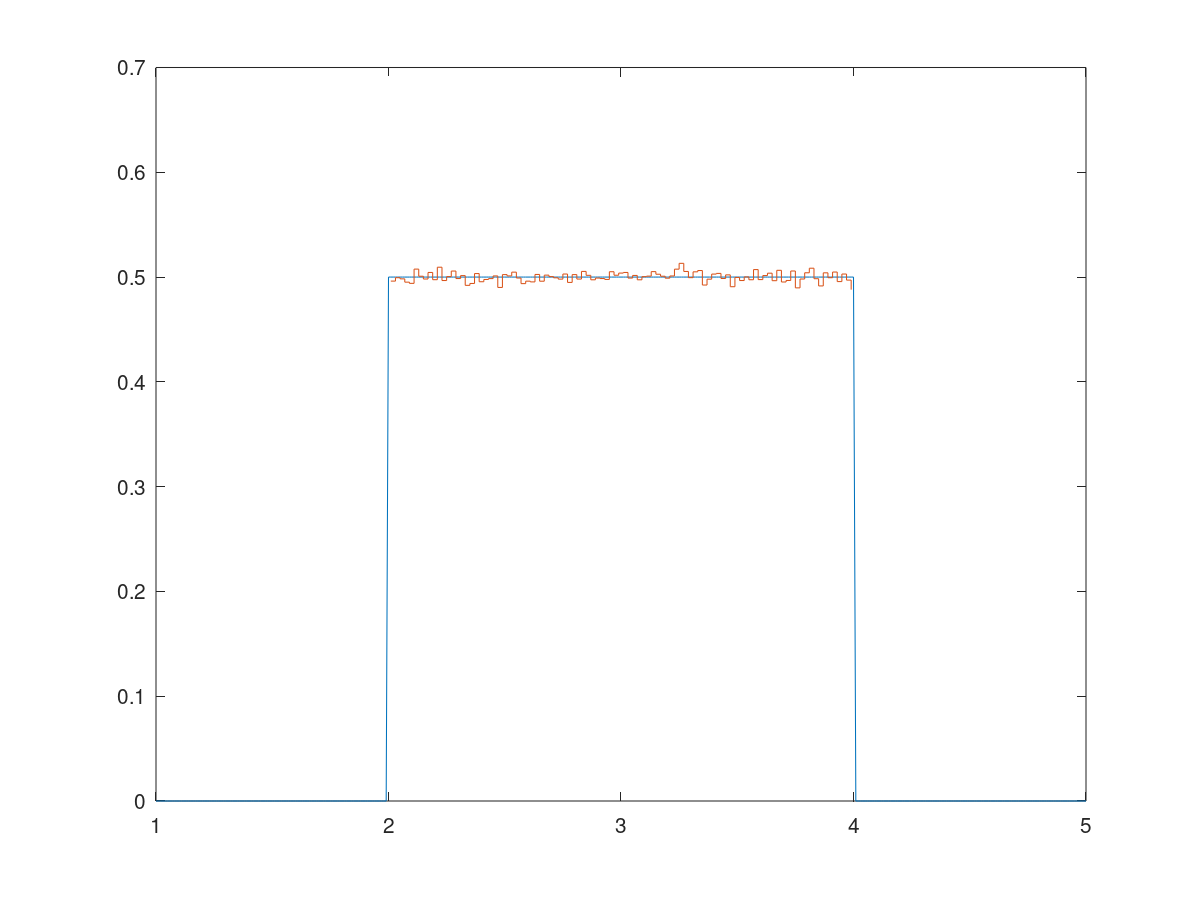
\includegraphics[width=0.9\linewidth]{hist.png}}
        	\end{figure}    
        \subsection{Нормальное распределение}
\begin{verbatim}
Expected alpha: 0.050000
Type I error alpha: 0.135000
Type I error alpha (corrected): 0.069000
Type II error beta with delta = 0.005000: 0.913000
Type II error beta with delta = 0.500000: 0.000000
\end{verbatim}
            \newpage
            \begin{figure}[h]
        	    \center{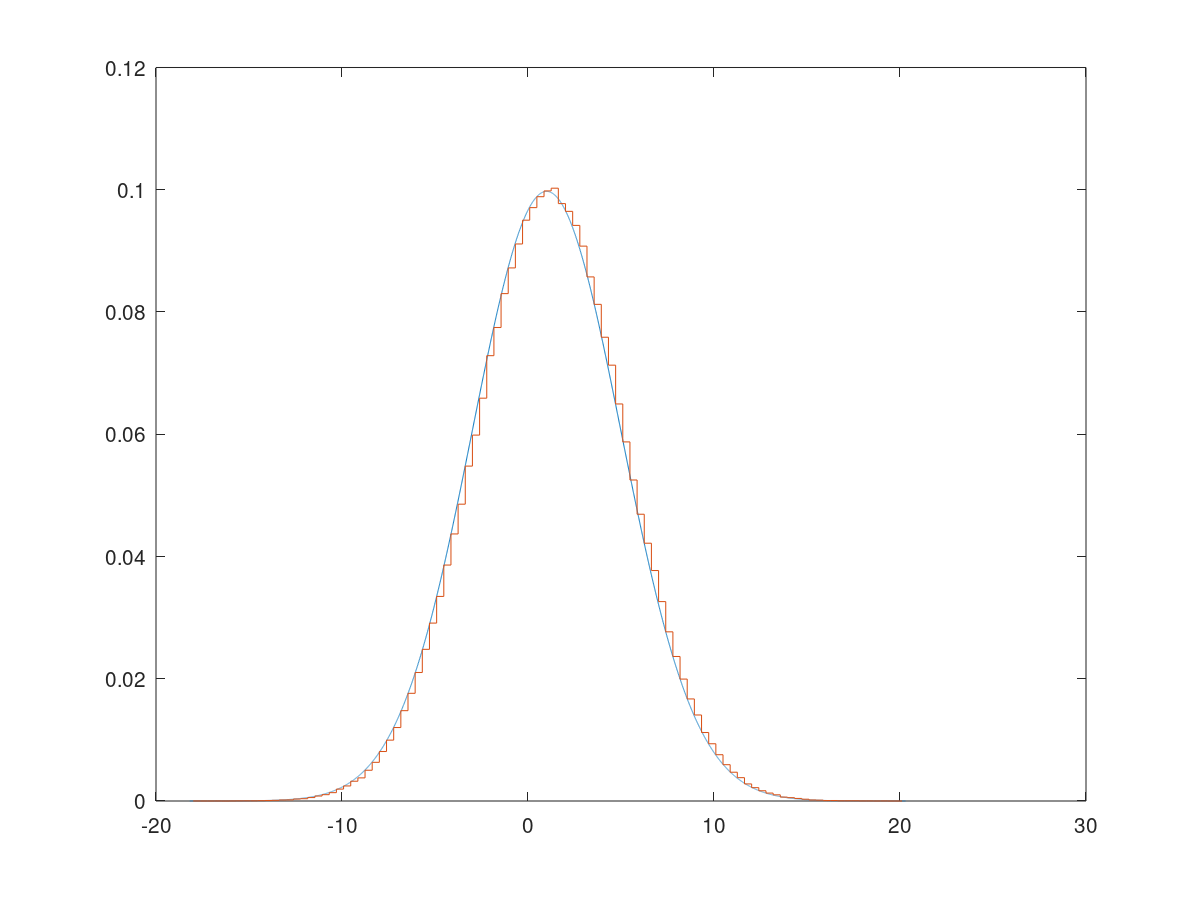
\includegraphics[width=0.9\linewidth]{graph_norm.png}}
        	\end{figure}                	
    \section{Вывод}
        Проверяя гипотезы по критерию хи-квадрат, установил, что значение оценки вероятности ошибки первого рода $\alpha$ отличает от теоретического на допустимую погрешность. По оценкам ошибки второго рода $\beta$ видно, что критерий хи-квадрат оказался чувствителен только к сильному изменению ($\delta = 0.5$), почти "не реагируя" на слабое ($\delta = 0.005$).
\end{document}
